\fenicschapter{Parallel Adaptive Mesh Refinement}
              {Parallel Adaptive Mesh Refinement}
              {Johan Hoffman, Johan Jansson and Niclas Jansson}
              {hoffman-4}

For many interesting problems one is often interested in rather
localized features of a solution, for example separation or transition
to turbulence in flow problems. It is often the case that it is to
expensive to uniformly refine a mesh to such an extent that these
features develops. The solution is to only refine the mesh in the
regions of most interest, or for example where the error is large.

This chapter is based on the work in \cite{Jan2008a}. First a brief
summary of the theory behind mesh refinement is given, followed by a
discussion of the issues with parallel refinement together with our
proposed solution. The chapter ends with a presentation of our
implementation of a fully distributed parallel adaptive mesh
refinement framework on a Blue Gene/L.

%------------------------------------------------------------------------------

\section{A brief overview of parallel computing}
\label{sect:para}

In this chapter, parallel computing refers to distributed memory
systems with message passing. It is assumed that the system is formed
by linking compute nodes together with some interconnect, in order to
form a virtual computer (or cluster) with a large amount of memory and
processors.

It is also assumed that the data, the mesh in this case is distributed
across the available processors. Shared entities are duplicated or
``ghosted'' on adjacent processors. In order to fully represent the
original mesh from the smaller distributed sub meshes, it is essential
that the information for the shared entities are the same for all
processors.

\section{Local mesh refinement}
\index{Adaptive mesh refinement}

Local mesh refinement has been studied by several authors over the
past years. The general idea is to split an element into a set of new
ones, with the constraint that the produced mesh must be
valid. Usually a mesh is valid if there are no ``hanging nodes'', that
is no node should be on another element's facet. How to split the
element in order to ensure this differs between different methods. One
common theme is edge bisection.

A common edge bisection algorithm bisects all edges in the element,
introducing a new vertex on each edge, and connecting them together to
form the new elements (see for example \cite{Bey1995a}). Other methods
bisect only one of the edges, which edge depends on the method. For
example one could select the edge which where most recently refined,
this method is often referred to as the newest vertex approach and
where described in \cite{Ebe1991a}. Another popular edge bisection
method is the longest edge \cite{Riv1984a}, where one always select
the longest edge for refinement. In order to ensure that the mesh is
free of ``hanging nodes'', the algorithm recursively bisects elements
until there are no ``hanging nodes'' left.

\subsection{The challenge of parallel mesh refinement}

Performing the refinement in parallel adds additional constraints on
the refinement method. Not only should the method prevent ``hanging
nodes'', it must also be guaranteed to terminate in a finite number of
steps.

In the parallel case, each processor owns a small part of the
distributed mesh. So if a new vertex is introduced on the boundary
between two processors, the algorithm must ensure that the information
propagates to all neighboring processors.

For an algorithm that bisects all edges in an element, the problem
reduces to a global decision problem, deciding which of the processors
information that should be used on all the other processors. But for
an algorithm that propagates the refinement like the longest edge, the
problem becomes a synchronization problem i) to detect and handle
refinement propagation between different processors and ii) to detect
global termination.

The first problem could easily be solved by dividing the refinement
into two different phases, one local refinement phase and one
propagation phase. In the first phase elements on the processor are
refined with an ordinary serial refinement method. This could create
non conforming elements on the boundary between processors. These are
fixed by propagating the refinement to the neighboring processor. This
is done in the second propagation phase. But since the next local
refinement phase could create an invalid mesh, one could get another
propagation phase and the possibility of another and so
forth. However, if the longest edge algorithm is used, termination is
guaranteed \cite{CasSav1999a}. But the problem is to detect when all
these local meshes are conforming, and also when they are conforming
at the same time, that means one has to detect global termination,
which is a rather difficult problem to solve efficiently, especially
for massively parallel systems for which we are aiming.

There has been some other work related to parallel refinement with
edge bisection. For example a parallel newest vertex algorithm has
been done by Zhang \cite{Zha2005a}. Since the algorithm does not need
to solve the termination detection problem, scaling is simply a
question of interconnect latency. Another work is the parallel longest
edge algorithm done by Casta\~nos and Savage \cite{CasSav1999a}. They
solve the termination detection problem with Dijkstras general
distributed termination algorithm, which simply detects termination by
counting messages sent and received from some controlling
processor. However, in both of these methods they only used a fairly
small amount of processors, less then one hundred, so it is difficult
to estimate how efficient and scalable these algorithms are. For more
processors the effects of communication cost and concurrency in the
communication patterns starts to be important, therefore we tried to
design an algorithm that would scale well for thousands of processors.

\subsection{A modified longest edge bisection algorithm}
\label{sect:modlong}

Instead of trying to solve the termination detection problem, one could try to modify the refinement algorithm in such a way that it would only require one synchronization step, thus less communication. With less communication overhead it should also scale better for a large number of processors.

\begin{figure}[htb]
 \psfrag{_1._}[l][bl][0.8]{1.}  \psfrag{_2._}[l][bl][0.8]{2.}
 \psfrag{_3._}[l][bl][0.8]{3.}  \begin{center}
 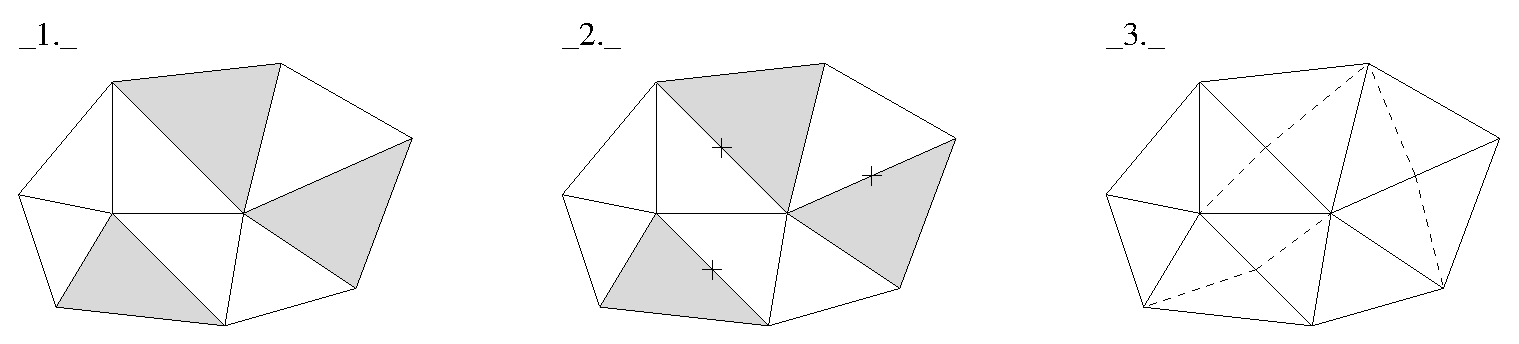
\includegraphics[width=1.0\columnwidth]{chapters/hoffman-4/eps/mref.eps}
 \end{center} \caption{An example of the refinement algorithm
 used. First a set of elements are marked for refinement (1). The
 longest edges are found (2), and all elements connected to these
 edges are finally bisected, the dashed lines in (3).}
 \label{fig:bisectexample}
\end{figure}

When this work started, DOLFIN did not have a pure longest edge
implementation. Instead of recursively fixing ``hanging nodes'' it
bisected elements in pairs (or groups) (see figure
\ref{fig:bisectexample}). Since this algorithm always terminate the
refinement by bisecting all elements connected to the refined edge, it
is a perfect candidate for an efficient parallel algorithm. If the
longest edge is shared by different processors, the algorithm must
only propagate the refinement onto all elements (processors) connected
to that edge, but then no further propagation is possible (see figure
\ref{fig:prop}).
\begin{figure}[htb]
 \psfrag{Cpu 0}[l][cl][0.7]{Cpu 0}
 \psfrag{Cpu 1}[l][cl][0.7]{Cpu 1}
 \psfrag{Cpu 2}[l][cl][0.7]{Cpu 2}
  \begin{center}
    \includegraphics[width=0.95\columnwidth]{chapters/hoffman-4/eps/prop.eps}
  \end{center}
   \caption{An example of the two simple cases of propagation. The dashed lines refers to how the processors wants to bisect the elements.}
   \label{fig:prop}
\end{figure}

However, notifying an adjacent processor of propagation does not solve
the problem entirely. As mentioned in section \ref{sect:para}, all
mesh entities shared by several processors must have the same
information in order to correctly represent the distributed mesh. The
refinement process must therefore guarantee that all newly created
vertices are assigned the same unique information on all the
neighboring processors. Another problematic case arises when
processors refine the same edge and the propagation ``collides'' (see
figure \ref{fig:prop}). In this case the propagation is done
implicitly but the processors must decide which of the new information
to use.
\begin{figure}[htb]
 \psfrag{Cpu 0}[l][cl][0.7]{Cpu 0} \psfrag{Cpu 1}[l][cl][0.7]{Cpu 1}
 \psfrag{Cpu 2}[l][cl][0.7]{Cpu 2} \begin{center}
 \includegraphics[width=0.65\columnwidth]{chapters/hoffman-4/eps/propprob.eps}
 \end{center} \caption{An example of the problematic case with
 multiple propagations. The dashed lines refers to how the processors
 wants to bisect the elements.}  \label{fig:propprob}
\end{figure}

A more complicated case is when an element receives multiple
propagation (possibly from different processors) on different edges
(see figure \ref{fig:propprob}). Since the modified longest edge
algorithm only allows one edge to be bisected per element, one of the
propagations must be selected and the other one rejected. This however
adds a difficulty to the simple algorithm. First of all, how should
the processors decide upon which edge to be refined? Clearly this
could not be done arbitrarily since when a propagation is forbidden,
all refinement done around that edge must be removed. Thus, in the
worst case it could destroy the entire refinement.

To solve the edge selection problem perfectly one needs an algorithm
with a global view of the mesh. In two dimensions with a triangular
mesh, the problem could be solved rather simple since each propagation
could only come from two different edges (one edge is always facing
the interior). By exchanging the desired propagation edges processors
could match theirs selected edges with the propagated ones, in an
attempt to minimize the number of forbidden propagations. However, in
three dimensions the problem starts to be such complicated that
multiple exchange steps are needed in order to solve the
problem. Hence, it becomes too expensive to solve.

Instead we propose an algorithm which solves the problem using an edge
voting scheme. Each processor refines the boundary elements, find
their longest edge and cast a vote for it. These votes are then
exchanged between processors, which add the received votes to its own
set of votes. Now the refinement process restarts, but instead of
using the longest edge criteria, edges are selected depending on the
maximum numbers of votes. In the case of a tie, the edge is selected
depending on a random number assigned to all votes.

Once a set of edges has been selected from the voting phase the
actually propagation starts by exchanging these with the other
processors. However, the voting could fail to ``pair'' refinements
together. For example, an element could lie between two processors
which otherwise does not share any common face. Each of these
processors wants to propagate into the neighboring element but on
different edges (see figure \ref{fig:probmissing}). Since the
processors on the left and right side of the element do not receive
the edge vote from each other, the exchange of votes will in this case
not help with selecting an edge that would work for both processors.

\begin{figure}[htb]
 \psfrag{Cpu 0}[l][cl][0.7]{Cpu 0}
 \psfrag{Cpu 1}[l][cl][0.7]{Cpu 1}
 \psfrag{Cpu 2}[l][cl][0.7]{Cpu 2}
  \begin{center}
   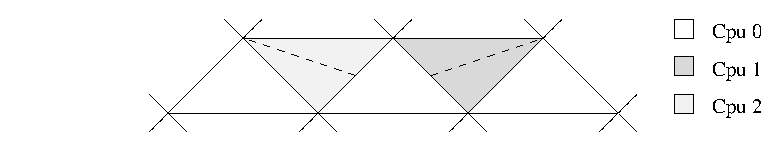
\includegraphics[width=0.65\columnwidth]{chapters/hoffman-4/eps/probmissing.eps}
  \end{center}
   \caption{An example of the case when edge votes could be missed. The dashed lines refers to how the processors wants to bisect the elements.}
   \label{fig:probmissing}

\end{figure}

To fix this, an additionally exchange step is needed and maybe another
and so forth, rendering the perfect fix impossible. Instead, the
propagation step ends by exchanging the refined edges which gave rise
to a forbidden propagation. All processors could then remove all
refinements that these edges introduced, and in the process, remove
any hanging nodes on the boundary between processors.

\section{The need of dynamic load balancing}
\index{Dynamic load balancing}

For parallel refinement, there is an additional problem not present in
the serial setting. As one refines the mesh, new vertices are added
arbitrarily at any processor. Thus, rendering an initially good load
balance useless. Therefore, in order to sustain a good parallel
efficiency the mesh must be repartitioned and redistributed after each
refinement, in other words dynamic load balancing is needed.

\begin{figure}[bt]
\begin{center}
  \includegraphics[width=0.49\columnwidth]{chapters/hoffman-4/eps/cr.eps}
  \includegraphics[width=0.49\columnwidth]{chapters/hoffman-4/eps/cr2.eps}
\end{center}
\caption{An example of load balancing were the locality of the data is considered. The mesh is refined three times around the cylinder, and for each step load balancing is performed, shading refers to processor id.}
\end{figure}

In the worst case, the load balancing routine must be invoked every
time a mesh is adapted, it has to be rather efficient, and for our
aim, scale well for a large number of processors. There are mainly two
different load balancing methods used today, diffusive and remapping
methods. Diffusive methods, like the physical meaning, by finding a
diffusion solution a heavily loaded processor's vertices would move to
another processor and in that way smear out the imbalance, described
for example in \cite{HuBla1995a, SchKar1997a}. Remapping methods,
relies on the partitioner's efficiency of producing good partitions
from an already partitioned dataset. In order to avoid costly data
movement, a remapping method tries to assign the new partitions to
processors in an optimal way. For problems where the imbalance occurs
rather localized, the remapping methods seems to perform better
\cite{SchKar1998a}. Hence, it maps perfectly to the localized
imbalance from local mesh refinement.

In this work, we used the load balancing framework of PLUM
\cite{Oli1998a} a remapping load balancer. The mesh is repartitioned
according to an imbalance model. Repartitioning is done before
refinement, this would in theory minimize data movement and speedup
refinement, since a more balanced number of element would be bisected
on each processor.

\subsection{Workload modelling}

The workload is modelled by a weighted dual graph of the mesh. Let
$G=(V,E)$ be the dual graph of the mesh, $q$ be one of the partitions
and let $w_i$ bet the computational work (weights) assigned to each
graph vertex. The processor workload is then defined as
\begin{equation}
  \label{eq:compwork}
  W(q) = \sum_{\forall w_i \in q} w_i
\end{equation}
where communication costs are neglected. Let $W_{avg}$ be the average workload and $W_{max}$ be the maximum, then the graph is considered imbalanced if 
\begin{equation}
  \label{eq:imbalancefactor}
  W_{max} /  W_{avg}  > \kappa
  %      \frac{W_{max}}{ W_{avg}}   > \epsilon
\end{equation}
where the threshold value $\kappa$ is based on the problem or machine characteristics. 

This model suits the modified longest edge algorithm (section
\ref{sect:modlong}) perfectly. Since the modifications reduces the
algorithm to only have one propagation and/or synchronization
step. The workload calculation becomes a local problem, thus it is
rather cheap to compute. So if we let each element represent one unit
of work, a mesh adapted by the modified algorithm would produce a dual
graph with vertex weights equal to one or two. Each element is only
bisected once, giving a computational weight of two elements for each
element marked for refinement.

\subsection{Remapping strategies}
\label{sect:intemap}

Remapping of the new partitions could be done in numerous ways,
depending on what metric one tries to minimize. Usually one often
talks about the two metrics \textsc{TotalV} and
\textsc{MaxV}. \textsc{MaxV} tries to minimize the redistribution time
by lowering the flow of data, while \textsc{TotalV} lower the
redistribution time by trying to keep the largest amount of data
local, for a more detailed description see \cite{Oli1998a}. We have
chosen to focus on the \textsc{TotalV} metric, foremost since it much
cheaper to solve then \textsc{MaxV}, and it produces equally good (or
even better) balanced partitions.

Independent of which metric one tries to solve. The result from the repartitioning is placed in a similarity matrix $S$, where each entry $S_{i,j}$ is the number of vertices on processor $i$ which would be placed in the new partition $j$. In our case, we want to keep the largest amount of data local, hence to keep the maximum row entry in $S$ local. This could be solved by transforming the matrix $S$ into a bipartite graph where each edge $e_{i,j}$ is weighted with $S_{i,j}$, the problem then reduces to the maximally weighted bipartite graph problem \cite{Oli1998a}.
\index{Parallel radix sort}

\section{The implementation on a massively parallel system}

The adaptive refinement method described in this chapter was
implemented using an early parallel version of DOLFIN, for a more
detailed description see \cite{Jan2008a}. Parallelization was
implemented for a message passing system, and all the algorithms were
designed to scale well for a large number of processors.

The challenge of implementing a refinement algorithm on a massively
parallel system is as always the communication latency. In order to
avoid that the message passing dominates the runtime, it is important
that the communication is kept at a minimum. Furthermore, in order to
obtain a good parallel efficiency, communication patterns must be
design in such way that they are highly concurrent, reducing
processors idle time etc.

\subsection{The refinement method}

Since element bisection is a local problem, without any communication,
the only part of the refinement algorithm that has to be well designed
for a parallel system is the communication pattern used for refinement
propagation.

For small scale parallelism, one could often afford to do the naive
approach, loop over all processors and exchange messages without any
problem. When the number of processors are increased, synchronization,
concurrency and deadlock prevention starts to become important factors
to considered when designing the communication pattern. A simple and
reliable pattern is easily implemented as follows. If the processors
send data to the left and receive data from the right in a circular
pattern, all processors would always be busy sending and receiving
data, thus no idle time.
\begin{algorithm}
%  \begin{algorithmic}
%    \FOR { i =1 \textbf{to} p-1}
%    \STATE src $\leftarrow$ (rank - 1 + p) $\mod$ p
%    \STATE dest $\leftarrow$ (rank + 1) $\mod$ p
%    \STATE sendrecv(send sendbuff(dest) to dest and recv from src)
%    \ENDFOR
%  \end{algorithmic}
  \caption{Communication pattern}
  \label{alg:cpattern}
\end{algorithm}

\editornote{Package \texttt{algorithmic.sty} conflicts with \texttt{algorithmicx.sty}.
Sort out which packages to use for algorithms.}

The refinement algorithm outlined in \ref{sect:modlong} is easily
implemented as a loop over all elements marked for refinement. For
each element marked for refinement it finds the longest edge and
bisect all elements connected to that edge. However, since an element
is only allowed to be bisected once, the algorithm is only allowed to
select the longest edge which is part of an unrefined element. In
order to make this work in parallel, one could structure the algorithm
in such a way that it first refines the shared elements, and propagate
the refinement. After that it could refine all interior elements
without any communication.
\begin{algorithm}
%  \begin{algorithmic}
%    \STATE refine shared entities
%    \FORALL {$c \in \mathcal{R}$}
%    \STATE find longest edge $e$ not marked as forbidden
%    \FORALL {elements $c_1$ connected to $e$}
%    \STATE bisect element $c_1$
%    \ENDFOR
%    \ENDFOR
%  \end{algorithmic}
  \caption{Refinement algorithm}
  \label{alg:ref}
\end{algorithm}

\editornote{Package \texttt{algorithmic.sty} conflicts with \texttt{algorithmicx.sty}.
Sort out which packages to use for algorithms.}

If we let $\mathcal{B}$ be the set of elements on the boundary between
processors, $\mathcal{R}$ the set of elements marked for
refinement. Then by using algorithm \ref{alg:cpattern} we could
efficiently express the refinement of shared entities in algorithm
\ref{alg:ref} with algorithm \ref{alg:pref}.
\begin{algorithm}
%  \begin{algorithmic}
%    \FORALL { $c \in \mathcal{B} \cup \mathcal{R}$}
%    \STATE find longest edge $e$
%    \IF {$e$ is on the boundary}
%    \STATE vote($e$) $\leftarrow$ vote($e$) + 1
%    \ENDIF
%    \ENDFOR
%    \STATE exchange votes with algorithm \ref{alg:cpattern}
%    \STATE mark all elements $\in \mathcal{B}$ with the maximum number of votes for refinement
%%    \FORALL {received votes on edge $e$} \STATE increase vote($e$) \ENDFOR
%%    \FORALL {$c \in \mathcal{B}$} \STATE mark $ \max_{e \in c}\left( \textrm{vote}(e) \right)$ for refinement \ENDFOR
%    \STATE exchange refinement with algorithm \ref{alg:cpattern}
%    \FORALL {received refinement} 
%    \IF {$e$ is not refined and not part of a refined element}
%    \STATE mark edge and propagate refinement
%    \ELSE
%    \STATE send back illegal propagation
%    \ENDIF
%    \ENDFOR
%    \FORALL {received illegal propagations}
%    \STATE remove refinement and hanging nodes
%    \ENDFOR
%  \end{algorithmic}
  \caption{Refinement of shared entities}
  \label{alg:pref}
\end{algorithm}

\editornote{Package \texttt{algorithmic.sty} conflicts with \texttt{algorithmicx.sty}.
Sort out which packages to use for algorithms.}

\subsection{The remapping scheme}

The maximally weighted bipartite graph problem for the \textsc{TotalV}
metric could be solved in an optimal way in $O(V^2 \log V + V E)$
steps \cite{Oli1998a}. Recall that the vertices in the graph are the
processors. Calculating the remapping could therefore become rather
expensive if a large number of processors are used. Since the solution
does not need to be optimal, a heuristic algorithm with a runtime of
$O(E)$ was used.

The algorithm starts by generating a sorted list of the similarity
matrix $S$. It then steps through the list and selects the largest
value which belongs to an unassigned partition. It was proven in
\cite{Oli1998a} that the algorithm's solution is always greater than
half of the optimal solution, thus it should not be a problem to solve
the remapping problem in a sub optimal way. Sorting was implemented
(as in the original PLUM paper) by a serial binary radix sort (the
matrix $S$ were gathered onto one processor), performing $\beta$
passes and using $2^r$ ``buckets'' for counting. In order to save some
memory the sorting was performed per byte of the integer instead of
the binary representation. Since each integer is represented by 4
bytes (true even for most 64-bits architectures) the number of passes
required was $\beta = 4$, and since each byte have 8 bits the number
of ``buckets'' needed were $2^8$.

However, since the similarity matrix $S$ is of the size $P \times P$
where $P$ is the number of processors, the sorting will have a runtime
of $O(P^2)$. This should not cause any problem on a small or medium
size parallel computer, as the one used in the fairly old PLUM
paper. But after 128-256 processors the complexity of the sorting
starts to dominates in the load balancer. To solve this problem,
instead of sorting $S$ on one processor we implemented a parallel
binary radix sort. The unsorted data of length $N$ was divided into
$N/P$ parts which were assigned to the available processors. The
internal $\beta$ sorting phases were only modified with a parallel
prefix calculation and a parallel swap phase (when the elements are
moved to the new ``sorted'' locations).
\begin{algorithm}
%  \begin{algorithmic}
%    \FOR {i = 0 to $\beta$} 
%    \FOR {j = 0 to N}
%    \STATE count[i byte of data(j)] $\leftarrow$ count[i byte of data(j)] + 1
%    \ENDFOR
%    \STATE count $\leftarrow$ Allreduce(count)
%    \FOR {j = 0 to $2^r$}
%    \STATE index(j) $\leftarrow$ ParallelPrefix(count(j))
%    \ENDFOR
%    \STATE redistribute elements according to index
%    \ENDFOR
%  \end{algorithmic}
  \caption{Parallel radix sort}
  \label{alg:pradix}
\end{algorithm}

\editornote{Package \texttt{algorithmic.sty} conflicts with \texttt{algorithmicx.sty}.
Sort out which packages to use for algorithms.}

\subsection{Theoretical and experimental analysis}

The adaptive refinement method described in this chapter has been
successfully tested on a 1024 node Blue Gene/L, each dual-processor
node could either be used to run two separate programs (virtual mode)
or run in coprocessor mode where one of the processor works as an
offload engine, for example handling parts of the message passing
stack \cite{GarBlu2005a, MorAlm2005a}.

As a test problem we used an unstructured mesh and refined all
elements inside a small local region, timed mesh refinement and load
balancing times. The problem were tested on $P = {32,128,512}$ nodes
both in virtual and coprocessor mode. Since the smallest number of
nodes that could be allocated was 32, all speedup results are
presented as a comparison against the time for 32 processors. To
capture possible communication bottlenecks, three different
unstructured meshes were used. First a cylinder mesh with $n_v =
566888$ vertices, secondly a hill with $n_V = 94720$ vertices and
finally, the cylinder again but with $n_v = 1237628$ vertices instead.
\begin{figure}[bt]
  \begin{center}
    \includegraphics[width=0.45\columnwidth]{chapters/hoffman-4/eps/cylmesh.eps}
    \includegraphics[width=0.45\columnwidth]{chapters/hoffman-4/eps/hillmesh2.eps}
  \end{center}
  \caption{Two of the meshes used during evaluation.}
\end{figure}

The regions selected for refinement were around the cylinder and
behind the hill. Since these regions already had the most number of
elements in the mesh, refinement would certainly result in an workload
imbalance. Hence, trigger the load balancing algorithms. In order to
analyze the experimental results we used a performance model which
decompose the total runtime $T$ into one serial computational cost
$T_{comp}$, and a parallel communication cost $T_{comm}$.
\begin{equation}
  T = T_{comp} + T_{comm}
\end{equation}

The mesh refinement has a local computational costs consisting of
iterating over and bisecting all elements marked for refinement, for a
mesh with $N_c$ elements $O(N_c/P)$ steps. Communication only occurs
when the boundary elements needs to be exchanged. Thus, each processor
would in the worst case communicate with $(P-1)$ other processors. If
we assume that there are $N_s$ shared edges, the total runtime with
communication becomes,
\begin{equation}
\label{eq:refine_time}
  T_{refine} = O\left(\frac{N_c}{P} \right) \tau_f + (P-1)(\tau_s + N_s \tau_b)
\end{equation}
where $\tau_f$ is the time to perform one (floating point) operation,
$\tau_s$ is the latency and $\tau_b$ the bandwidth. So based on the
performance model, more processors would lower the computational time,
but in the same time increase the communication time.

The most computationally expensive part of the load balancer is the
remapping or assignment of the new partitions. As discussed earlier,
we used an heuristic with a runtime of $O(E)$, the number of edges in
the bipartite graph. Hence, in the worst case $ E \approx P^2$. The
sorting phase is linear, and due to the parallel implementation it
runs in $O(P)$. Communication time for the parallel prefix calculation
is given by, for $m$ data it sends and calculates in $m/P$
steps. Since the prefix consists of $2^r$ elements, it would take
$2^r/P$ steps, and we have to do this for each $\beta$ sorting
phases. In the worst case the reordering phase (during sorting) needs
to send away all the elements, thus $P$ communication steps, which
gives the total runtime.
\begin{equation}
  \label{eq:load_time}
  T_{loadb} = O(P^2) \tau_f + \beta \left( \tau_s + \left( \frac{2^r}{P} + P \right) \tau_b \right)
\end{equation}

According to this, load balancing should not scale well for a large
number of processors (due to the $O(P^2)$ term). However the more
realistic average case should be $O(P)$. So again, with more
processors the runtime could go up due to the communication cost.

If we then compare with the experimental results presented in figure
\ref{fig:refsp}, we see that the performance degenerates when a large
number of processors are used. The question is why? Is it solely due
to the increased communication cost? Or is the load balancer's
computational cost to blame?
\begin{figure}[hbt]
  \psfrag{r}[c][l][0.75]{Speedup}
  \psfrag{p}[c][c][0.75]{Number of processors}
  \psfrag{1}[c][c][0.7]{1}
  \psfrag{2}[c][c][0.7]{2}
  \psfrag{3}[c][c][0.7]{3}
  \psfrag{4}[c][c][0.7]{4}
  \psfrag{5}[c][c][0.7]{5}
  \psfrag{6}[c][c][0.7]{6}
  \psfrag{7}[c][c][0.7]{7}
  \psfrag{8}[c][c][0.7]{8}

  \psfrag{32}[c][c][0.7]{32}
  \psfrag{64}[c][c][0.7]{64}
  \psfrag{128}[c][c][0.7]{128}
  \psfrag{256}[c][c][0.7]{256}
  \psfrag{512}[c][c][0.7]{512}
  \psfrag{1024}[c][c][0.7]{1024}

  \psfrag{cyl1}[c][c][0.7]{cyl1}
  \psfrag{cyl2}[c][c][0.7]{cyl2}
  \psfrag{hill}[c][c][0.7]{hill}

  \begin{center}
      \includegraphics[width=0.55\columnwidth]{chapters/hoffman-4/eps/speedup.eps}
      \caption{Refinement speedup (incl. load balancing)}
      \label{fig:refsp}
  \end{center}
\end{figure}

First of all one could observe that when the number of elements per
processor is small. The communication costs starts to dominate, see
for example the results for the smaller hill mesh (represented by a
triangle in the figure). The result is better for the medium size
cylinder (represented by a diamond), and even better for the largest
mesh (represented by a square). If the load balancing time was the
most dominating part, a performance drop should have been observed
around 128 - 256 processors. Instead performance generally drops after
256 processors. A possible explanation for this could be the small
amount of local elements. Even for the larger $10^6$ element mesh,
with 1024 processors the number of local elements is roughly $10^3$,
which is probably too few to balance the communication costs.

This illustrate the curse of massively parallel, distributed memory
systems. In order to gain anything from the large amount of
processors, either one has to have a large local computational cost,
or one has to increase the dataset in order to mask the communication
latency. To illustrate how large the mesh needs to be, we uniformly
refined the larger cylinder, locally refined the same region as before
and timed it for 256,512 and 1024 processors. Now the refinement
performance better, as can be seen in table \ref{tab:reftime}. But
again performance drops between 512 and 1024 processors.
\begin{table}[t]
  \begin{center}
    \begin{tabular}{|c|c|c|}
      \hline
      Processors & Execution time & Speedup \\
      \hline
      256 & 33.50 & 1.0 \\
      512 & 23.19 & 1.44 \\
      1024 & 19.24 & 1.74 \\
      \hline
    \end{tabular}
  \end{center}
  \caption{\label{tab:reftime} Refinement time for a nine million vertices mesh}
\end{table}

However, despite the decrease in speedup, one could see that the
algorithm seems to scale well, given that the local amount of elements
are fairly large. It is close to linear scaling from 32 to 256
processors, and we see no reason for it to not scale equally good
between 256 and 1024 processors, given that the local part of the mesh
is large enough.

\section{Summary and outlook}

In this chapter we presented some of the challenges with parallel mesh
refinement. How these could be solved and finally how these solutions
were implemented for a distributed memory system. In the final section
some theoretical and experimental performance results were presented
and explained. One could observe how well the implementation performs,
until the curse of slow interconnect starts to affect the results.

One aspect of the refinement problem that has not been touched upon in
this chapter is the mesh quality. The modification done to the longest
edge algorithm (see section \ref{sect:modlong}), unfortunately
destroys the good properties of the original recursive algorithm. It
was a trade off between efficiency and mesh quality. As mentioned
before, the problem with the original algorithm is the efficiency of
propagation and global termination detection. Currently our work is
focused in overcoming these problems, implementing an efficient
parallel refinement method with good quality aspects, which also
performs well for thousands of processors.
